\documentclass[a4paper,14pt]{extarticle}

\usepackage[a4paper,margin=2.5cm]{geometry}
\usepackage{iftex}
\ifPDFTeX
  \usepackage[T2A]{fontenc}
  \usepackage[utf8]{inputenc}
  \usepackage[russian]{babel}
  \usepackage{tempora}
\else
  \usepackage[russian]{babel}
  \usepackage{fontspec}
  \setmainfont{Times New Roman}
\fi

\usepackage{amsmath}
\usepackage{amssymb}
\usepackage{array}
\usepackage{booktabs}
\usepackage{caption}
\usepackage{float}
\usepackage{graphicx}
\usepackage{longtable}
\usepackage[unicode,colorlinks=true,linkcolor=blue,urlcolor=magenta]{hyperref}
\usepackage{listings}
\usepackage{listingsutf8}
\usepackage{setspace}
\usepackage{xcolor}

\onehalfspacing
\renewcommand{\arraystretch}{1.15}

\definecolor{codegreen}{rgb}{0,0.6,0}
\definecolor{codegray}{rgb}{0.5,0.5,0.5}
\definecolor{codepurple}{rgb}{0.58,0,0.82}
\definecolor{backcolour}{rgb}{0.95,0.95,0.92}

\lstset{
    language=Python,
    backgroundcolor=\color{backcolour},
    commentstyle=\color{codegreen},
    keywordstyle=\color{blue},
    numberstyle=\tiny\color{codegray},
    stringstyle=\color{codepurple},
    basicstyle=\ttfamily\small,
    breakatwhitespace=false,
    breaklines=true,
    captionpos=b,
    keepspaces=true,
    numbers=left,
    numbersep=5pt,
    showspaces=false,
    showstringspaces=false,
    showtabs=false,
    tabsize=2,
    frame=single,
    inputencoding=utf8,
    extendedchars=true,
    texcl=true,
    literate={а}{{\cyra}}1 {б}{{\cyrb}}1 {в}{{\cyrv}}1 {г}{{\cyrg}}1 {д}{{\cyrd}}1 {е}{{\cyre}}1 {ё}{{\"e}}1 {ж}{{\cyrzh}}1 {з}{{\cyrz}}1 {и}{{\cyri}}1 {й}{{\cyrishrt}}1 {к}{{\cyrk}}1 {л}{{\cyrl}}1 {м}{{\cyrm}}1 {н}{{\cyrn}}1 {о}{{\cyro}}1 {п}{{\cyrp}}1 {р}{{\cyrr}}1 {с}{{\cyrs}}1 {т}{{\cyrt}}1 {у}{{\cyru}}1 {ф}{{\cyrf}}1 {х}{{\cyrh}}1 {ц}{{\cyrc}}1 {ч}{{\cyrch}}1 {ш}{{\cyrsh}}1 {щ}{{\cyrshch}}1 {ъ}{{\cyrhrdsn}}1 {ы}{{\cyry}}1 {ь}{{\cyrsftsn}}1 {э}{{\cyrerev}}1 {ю}{{\cyryu}}1 {я}{{\cyrya}}1 {А}{{\CYRA}}1 {Б}{{\CYRB}}1 {В}{{\CYRV}}1 {Г}{{\CYRG}}1 {Д}{{\CYRD}}1 {Е}{{\CYRE}}1 {Ё}{{\"E}}1 {Ж}{{\CYRZH}}1 {З}{{\CYRZ}}1 {И}{{\CYRI}}1 {Й}{{\CYRISHRT}}1 {К}{{\CYRK}}1 {Л}{{\CYRL}}1 {М}{{\CYRM}}1 {Н}{{\CYRN}}1 {О}{{\CYRO}}1 {П}{{\CYRP}}1 {Р}{{\CYRR}}1 {С}{{\CYRS}}1 {Т}{{\CYRT}}1 {У}{{\CYRU}}1 {Ф}{{\CYRF}}1 {Х}{{\CYRH}}1 {Ц}{{\CYRC}}1 {Ч}{{\CYRCH}}1 {Ш}{{\CYRSH}}1 {Щ}{{\CYRSHCH}}1 {Ъ}{{\CYRHRDSN}}1 {Ы}{{\CYRY}}1 {Ь}{{\CYRSFTSN}}1 {Э}{{\CYREREV}}1 {Ю}{{\CYRYU}}1 {Я}{{\CYRYA}}1
}

\begin{document}
\pagenumbering{gobble}

\begin{titlepage}
    \centering

    \IfFileExists{../tex/lab3/fefu.jpg}{
        
\includegraphics[scale=0.15]{../tex/lab3/fefu.jpg}\\[0.4cm]
    }{
        \vspace*{1.8cm}
    }

    МИНИСТЕРСТВО НАУКИ И ВЫСШЕГО ОБРАЗОВАНИЯ\\
    РОССИЙСКОЙ ФЕДЕРАЦИИ\\
    Федеральное государственное автономное образовательное учреждение высшего образования\\
    \textbf{«Дальневосточный федеральный университет»}\\
    \textbf{(ДВФУ)}\\[0.3cm]
    \rule{\linewidth}{0.7mm}\\[0.3cm]

    \textbf{ИНСТИТУТ МАТЕМАТИКИ И КОМПЬЮТЕРНЫХ ТЕХНОЛОГИЙ}\\[0.3cm]
    \textbf{Кафедра математического и компьютерного моделирования}\\[0.9cm]

    Избосарова Жасмина Олимжоновна\\
    \textbf{ИДЗ №16}\\[0.3cm]

    Направление подготовки 02.03.01 СЦТ «Сквозные цифровые технологии»,\\
    образовательная программа «Математика и компьютерные науки»,\\
    очная форма обучения\\[1cm]

    \raggedleft
    \textbf{Студент группы Б9123-02.03.01сцт2}\\
    \rule{4.5cm}{0.3mm} Ж.\,О.~Избосарова\\[1cm]

    \textbf{Руководитель проекта}\\
    \rule{4.2cm}{0.3mm} К.\,А.~Ганжа

    \vfill
    \centering
    Владивосток\\
    2026
\end{titlepage}

\clearpage
\pagenumbering{arabic}

% \section{Введение}

% Расчёты, построение графиков и формирование таблиц выполнены скриптом \texttt{idz\_code.py}.
% Ниже приведены используемые формулы и итоговые численные результаты для варианта 16.

\section{Задача 1}

Условие:
\begin{itemize}
    \item дано: выборка объёма \(n=100\) из непрерывной случайной величины \(X_{16}\), см. Приложение~А, табл.~1;
    \item требуется: построить интервальный ряд, полигон частот, гистограмму и ЭФР, а также найти \(\overline{x}\) и \(s_n^2\).
\end{itemize}

Для интервального ряда используем формулу Стерджесса
\[
k = \left\lceil 1 + 3.322 \log_{10} n \right\rceil,
\qquad
\Delta = \frac{x_{\max} - x_{\min}}{k}.
\]
Частоты интервалов и их относительные частоты
\[
\omega_i = \frac{n_i}{n},
\qquad
h_i = \frac{\omega_i}{\Delta_i}.
\]
Эмпирическая функция распределения
\[
F_n(x)=\frac{1}{n}\sum_{i=1}^{n}\mathbf{1}\{X_i\le x\}.
\]
Выборочные характеристики
\[
\overline{x}=\frac{1}{n}\sum_{i=1}^{n}x_i,
\qquad
s_n^2=\frac{1}{n}\sum_{i=1}^{n}(x_i-\overline{x})^2.
\]

Для  выборки получено
\[
\overline{x}=0.2430,\qquad s_n^2=1.0276.
\]

\begin{table}[H]
\centering
\caption{Интервальный ряд для задачи 1}
\small
\begin{tabular}{cccc}
\toprule
Интервал & $n_i$ & $\omega_i$ & $h_i$ \\
\midrule
$[-2,53; -1,87)$ & 1 & 0,0100 & 0,0152 \\
$[-1,87; -1,21)$ & 7 & 0,0700 & 0,1061 \\
$[-1,21; -0,55)$ & 13 & 0,1300 & 0,1970 \\
$[-0,55; 0,11)$ & 22 & 0,2200 & 0,3333 \\
$[0,11; 0,77)$ & 25 & 0,2500 & 0,3788 \\
$[0,77; 1,43)$ & 19 & 0,1900 & 0,2879 \\
$[1,43; 2,09)$ & 9 & 0,0900 & 0,1364 \\
$[2,09; 2,75]$ & 4 & 0,0400 & 0,0606 \\
\bottomrule
\end{tabular}
\end{table}


\begin{figure}[H]
    \centering
    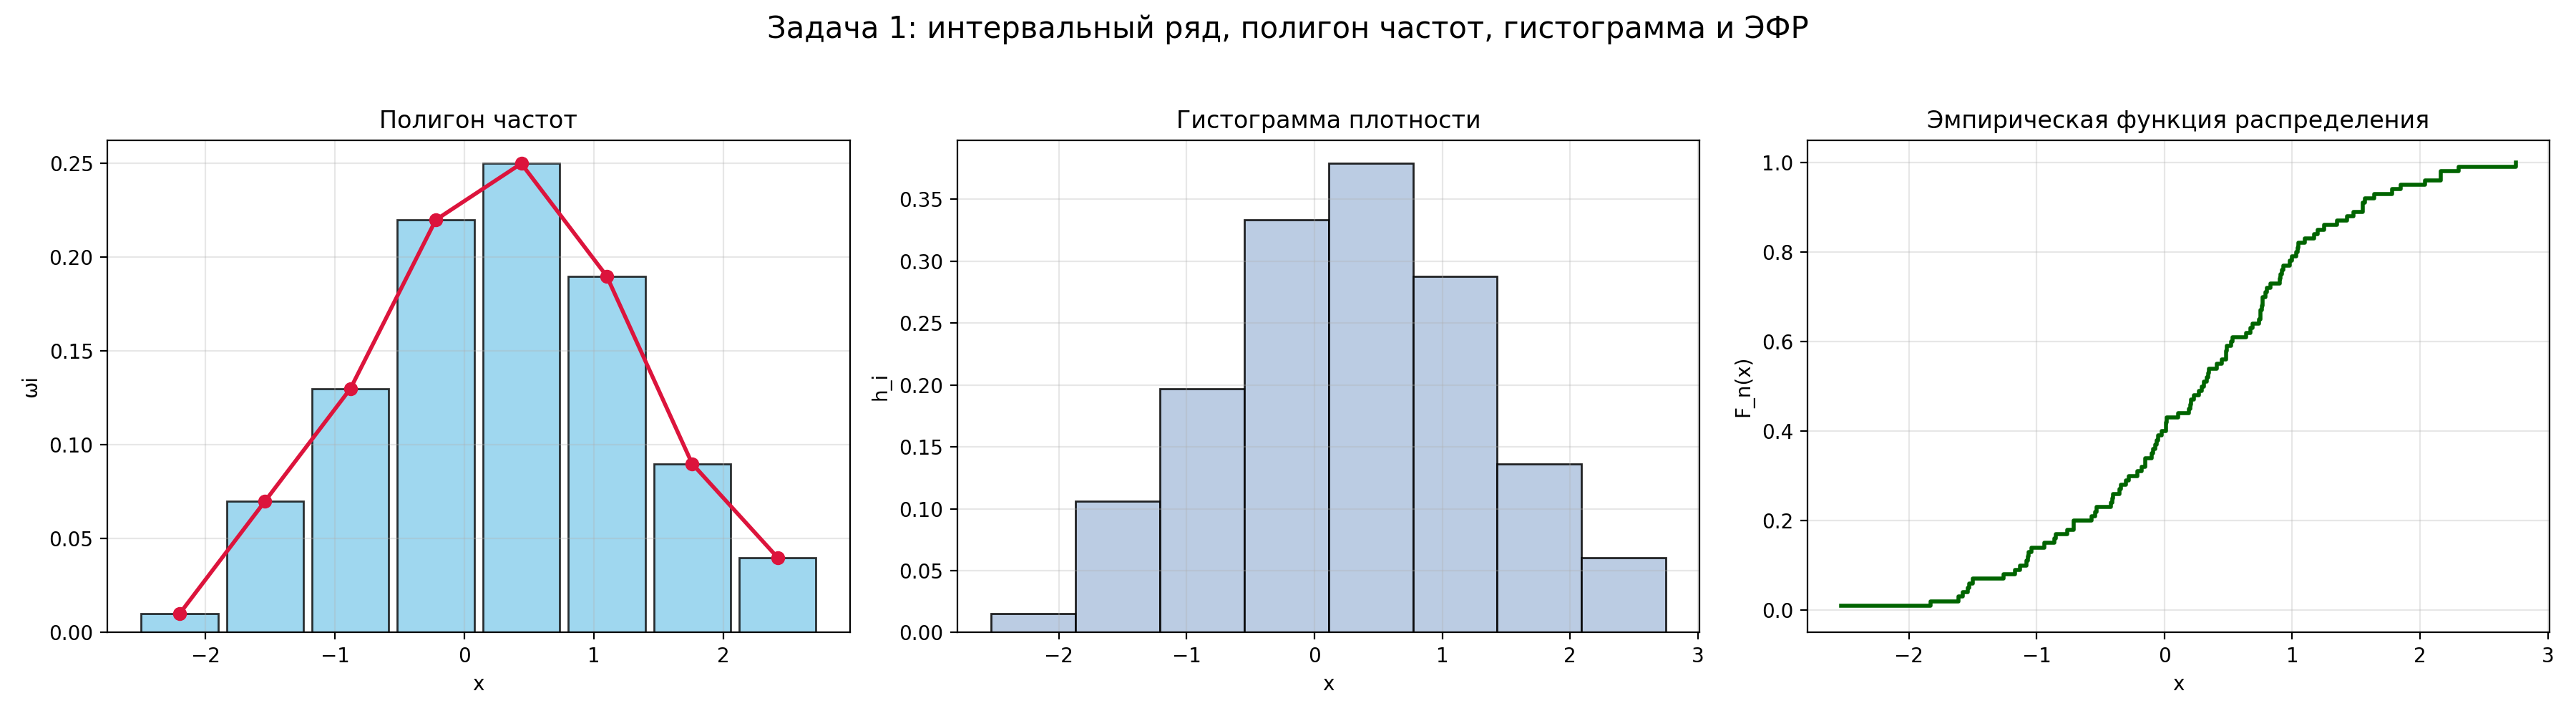
\includegraphics[width=\linewidth]{figures/task1_plots.png}
    \caption{Интервальный ряд, полигон частот, гистограмма и эмпирическая функция распределения}
\end{figure}

\subsection*{Использованный код}

\begin{lstlisting}
x = TASK1_SAMPLE
n = x.size
x_mean = float(np.mean(x))
x_var = float(np.mean((x - x_mean) ** 2))

k = max(1, math.ceil(1 + 3.322 * math.log10(n)))
edges = np.linspace(float(x.min()), float(x.max()), k + 1)
counts, _ = np.histogram(x, bins=edges)
widths = np.diff(edges)
rel = counts / n
dens = rel / widths
sorted_x = np.sort(x)
ecdf = np.arange(1, n + 1) / n
\end{lstlisting}

\section{Задача 2}


\begin{itemize}
    \item дано: выборка \(X_1,\dots,X_n\) из гамма-распределения с известным \(\lambda\) и неизвестным \(\alpha\);
    \item требуется: найти оценку \(\alpha\) методом максимального правдоподобия и проверить её состоятельость и несмещённость.
\end{itemize}

Пусть плотность гамма-распределения имеет вид
\[
f_{\xi}(x)=\frac{\alpha^{\lambda}}{\Gamma(\lambda)}x^{\lambda-1}e^{-\alpha x},\qquad x>0,
\]
где \(\lambda\) известно, а \(\alpha\) неизвестно.

Функция правдоподобия
\[
L(\alpha)=\prod_{i=1}^{n}\frac{\alpha^{\lambda}}{\Gamma(\lambda)}X_i^{\lambda-1}e^{-\alpha X_i}.
\]
Логарифм правдоподобия
\[
\ell(\alpha)=n\lambda\ln\alpha-\alpha\sum_{i=1}^{n}X_i + C.
\]
Из уравнения
\[
\frac{d\ell}{d\alpha}=\frac{n\lambda}{\alpha}-\sum_{i=1}^{n}X_i=0
\]
получаем оценку максимального правдоподоби
\[
\hat{\alpha}_{\text{МП}}=\frac{n\lambda}{\sum_{i=1}^{n}X_i}=\frac{\lambda}{\overline{X}}.
\]

Проверка состоятельности
\[
\overline{X}\xrightarrow{P}\mathbb{E}X=\frac{\lambda}{\alpha}
\quad \Longrightarrow \quad
\hat{\alpha}_{\text{МП}}=\frac{\lambda}{\overline{X}}\xrightarrow{P}\alpha.
\]
Следовательно, оценка состоятельна

Проверка несмещённости
\[
\sum_{i=1}^{n}X_i \sim \Gamma(n\lambda,\alpha), \qquad
\mathbb{E}\!\left[\frac{1}{\sum_{i=1}^{n}X_i}\right]=\frac{\alpha}{n\lambda-1}, \quad n\lambda>1.
\]
Тогда
\[
\mathbb{E}\hat{\alpha}_{\text{МП}}
=n\lambda\,\mathbb{E}\!\left[\frac{1}{\sum_{i=1}^{n}X_i}\right]
=\alpha\,\frac{n\lambda}{n\lambda-1}\neq \alpha.
\]
Итак, оценка смещённая, но асимптотически несмещённая.

\section{Задача 3}

Условия
\begin{itemize}
    \item дано: выборка объёма \(n=36\) из нормальной случайной величины \(X_{16}\), см. Приложение~А, табл.~2;
    \item требуется: построить точные доверительные интервалы для параметров \(m\) и \(\sigma^2\) при \(\beta=0.89\).
\end{itemize}

Для нормальной выборки используем точные доверительные интервалы
\[
\frac{\overline{X}-m}{S/\sqrt{n}} \sim t_{n-1},
\qquad
\frac{(n-1)S^2}{\sigma^2}\sim \chi^2_{n-1},
\]

\[
S^2=\frac{1}{n-1}\sum_{i=1}^{n}(X_i-\overline{X})^2.
\]
При доверительной вероятности \(\beta=0.89\) имеем \(\alpha=1-\beta=0.11\)
тогда
\[
m \in \left(
\overline{X}-t_{1-\alpha/2;\,n-1}\frac{S}{\sqrt{n}},
\overline{X}+t_{1-\alpha/2;\,n-1}\frac{S}{\sqrt{n}}
\right),
\] 
\[
\sigma^2 \in \left(
\frac{(n-1)S^2}{\chi^2_{1-\alpha/2;\,n-1}},
\frac{(n-1)S^2}{\chi^2_{\alpha/2;\,n-1}}
\right).
\]

Для выборки из таблицы 2 получено:
\[
\overline{X}=11.6506,\qquad S^2=64.1813,\qquad t_{0.945;35}=1.6398.
\]

\begin{table}[H]
\centering
\caption{Точные доверительные интервалы для задачи 3}
\small
\begin{tabular}{cc}
\toprule
Параметр & Значение \\
\midrule
$n$ & 36 \\
$\overline{x}$ & 11,6506 \\
$S^2$ & 64,1813 \\
$t_{1-\alpha/2;\,n-1}$ & 1,6398 \\
$\chi^2_{\alpha/2;\,n-1}$ & 22,7556 \\
$\chi^2_{1-\alpha/2;\,n-1}$ & 49,3105 \\
ДИ для $m$ & [9,4610; 13,8401] \\
ДИ для $\sigma^2$ & [45,5551; 98,7160] \\
ДИ для $\sigma$ & [6,7495; 9,9356] \\
\bottomrule
\end{tabular}
\end{table}


\section{Задача 4}

Условия
\begin{itemize}
    \item дано: \(n=20\) измерений нормальной совокупности и несмещённая выборочная дисперсия \(s^2\);
    \item требуетс найти вероятность того, что относительная погрешность оценки дисперсии не превышает \(0.3\).
\end{itemize}

Если
\[
\frac{(n-1)s^2}{\sigma^2}\sim\chi^2_{n-1},
\]
то относительная ошибка оценки дисперсии не превышает \(0.3\) при
\[
0.7\sigma^2 \le s^2 \le 1.3\sigma^2.
\]
Следовательно,
\[
P\left(0.7(n-1)\le \chi^2_{n-1}\le 1.3(n-1)\right)
\]
для \(n=20\) и \(n-1=19\) равна
\[
P \approx 0.6522.
\]

\begin{table}[H]
\centering
\caption{Ответ к задаче 4}
\small
\begin{tabular}{cc}
\toprule
Параметр & Значение \\
\midrule
$n$ & 20 \\
$\nu = n-1$ & 19 \\
$\varepsilon$ & 0,3000 \\
$P\{|s^2-\sigma^2|/\sigma^2 \le 0{,}3\}$ & 0,6522 \\
\bottomrule
\end{tabular}
\end{table}


\section{Задача 5}

Условие
\begin{itemize}
    \item дано x частоты попаданий в интервалы и гипотетическая плотность;
    \item требуетс  проверить гипотезу по критерию Пирсона при \(\alpha=0.01\) и указать достигнутый уровень значимости.
\end{itemize}

Плотность
\[
f(x)=\frac{1}{2\sqrt{\pi}}e^{-\frac{(x-2)^2}{4}}
\]
соответствует нормальному закону \(N(2,2)\), так как
\[
\frac{1}{\sqrt{2\pi\sigma^2}}e^{-\frac{(x-\mu)^2}{2\sigma^2}}
\quad \Rightarrow \quad
\mu=2,\ \sigma^2=2.
\]
Теоретические вероятности по интервалам
\[
p_k = P(a_k<X<b_k)=\Phi\!\left(\frac{b_k-2}{\sqrt{2}}\right)-\Phi\!\left(\frac{a_k-2}{\sqrt{2}}\right).
\]
Статистика Пирсона
\[
\chi^2_{\text{набл}}=\sum_{k=1}^{r}\frac{(n_k-np_k)^2}{np_k}.
\]

В данной задаче по шести классам получено
\[
\chi^2_{\text{набл}}=7.9669,\qquad
\chi^2_{0.99;5}=15.0863,\qquad
p\text{-value}=0.1581.
\]
Следовательно при уровне значимости \(0.01\) гипотеза о соответствии не отвергается.
Сумма теоретических вероятностей по данным классам равна \(0.9661\).

\begin{table}[H]
\centering
\caption{Проверка гипотезы по критерию Пирсона для задачи 5}
\small
\begin{tabular}{ccccc}
\toprule
Интервал & $n_k$ & $p_k$ & $n p_k$ & $\frac{(n_k-np_k)^2}{np_k}$ \\
\midrule
$(-1; 0)$ & 6 & 0,0617 & 4,3192 & 0,6541 \\
$(0; 1)$ & 11 & 0,1611 & 11,2770 & 0,0068 \\
$(1; 2)$ & 17 & 0,2602 & 18,2175 & 0,0814 \\
$(2; 3)$ & 13 & 0,2602 & 18,2175 & 1,4943 \\
$(3; 4)$ & 14 & 0,1611 & 11,2770 & 0,6575 \\
$(4; 5)$ & 9 & 0,0617 & 4,3192 & 5,0728 \\
Итого & 70 & 0,9661 & 67,6274 & 7,9669 \\
\bottomrule
\end{tabular}
\end{table}


\section{Задача 6}

Условие
\begin{itemize}
    \item дано: две независимые нормальные выборки объёмов \(n_x=15\) и \(n_y=13\), их средние и исправленные дисперсии;
    \item требуется: проверить гипотезу \(H_0:m_x=m_y\) против \(H_1:m_x>m_y\) при \(\alpha=0.025\).
\end{itemize}

При предположении равенства неизвестных дисперсий используем объединённую оценку
\[
S_p^2=\frac{(n_x-1)s_x^2+(n_y-1)s_y^2}{n_x+n_y-2}.
\]
Статистика критерия:
\[
T=\frac{\overline{X}-\overline{Y}}{S_p\sqrt{\frac{1}{n_x}+\frac{1}{n_y}}}
\sim t_{n_x+n_y-2}.
\]
Для альтернативы \(H_1:m_x>m_y\) отвергаем \(H_0\), если
\[
T>t_{1-\alpha;\,n_x+n_y-2}.
\]

В задаче получено
\[
T_{\text{набл}}=2.2222,\qquad t_{0.975;26}=2.0555,\qquad p=0.0176.
\]
Следовательно, гипотеза \(H_0:m_x=m_y\) отвергается в пользу \(H_1:m_x>m_y\).

\begin{table}[H]
\centering
\caption{Проверка гипотезы о равенстве средних для задачи 6}
\small
\begin{tabular}{cc}
\toprule
Параметр & Значение \\
\midrule
$n_x$ & 15 \\
$n_y$ & 13 \\
$\overline{x}$ & 3,8000 \\
$\overline{y}$ & 3,5000 \\
$s_x^2$ & 0,1500 \\
$s_y^2$ & 0,1000 \\
$s_p^2$ & 0,1269 \\
$T_{\text{набл}}$ & 2,2222 \\
$t_{1-\alpha;\,n_x+n_y-2}$ & 2,0555 \\
$p$-value & 0,0176 \\
\bottomrule
\end{tabular}
\end{table}


\section{Задача 7}

Условие
\begin{itemize}
    \item дано: 40 пар наблюдений \((X,Y)\), см. Приложение~А, табл.~3;
    \item требуется: построить корреляционное поле, найти линейную и квадратичную регрессии, проверить значимость коэффициентов и сравнить модели.
\end{itemize}

Для линейной регрессии
\[
\hat y = \beta_0+\beta_1x
\]
оценки МНК можно записать как
\[
\hat\beta_1=\frac{\sum_{i=1}^{n}(x_i-\overline{x})(y_i-\overline{y})}{\sum_{i=1}^{n}(x_i-\overline{x})^2},
\qquad
\hat\beta_0=\overline{y}-\hat\beta_1\overline{x}.
\]

Для квадратичной модели
\[
\hat y = \beta_0+\beta_1x+\beta_2x^2
\]
вектор оценок находится по формуле
\[
\hat\beta=(X^TX)^{-1}X^Ty.
\]

Проверка значимости коэффициентов:
\[
t_j=\frac{\hat\beta_j}{\sqrt{\hat\sigma^2\left[(X^TX)^{-1}\right]_{jj}}},
\qquad
\hat\sigma^2=\frac{\sum e_i^2}{n-p}.
\]
Коэффициент считается значимым, если
\[
|t_j|>t_{1-\alpha/2;\,n-p},
\qquad \alpha=0.075.
\]

Для сравнения моделей используем
\[
\hat\sigma^2_{\text{ост}}=\frac{\sum e_i^2}{n-p},
\qquad
R^2=1-\frac{\sum e_i^2}{\sum (y_i-\overline{y})^2}.
\]

По данным задачи получено
\[
\hat\beta^{(1)}_0=37.8035,\quad \hat\beta^{(1)}_1=-0.1556,
\]
\[
\hat\beta^{(2)}_0=38.2925,\quad \hat\beta^{(2)}_1=-0.2932,\quad \hat\beta^{(2)}_2=0.0067.
\]
Обе модели имеют очень малый коэффициент детерминации, значит зависимость слабая.
По остаточной дисперсии лучше линейная модель, так как
\[
\hat\sigma^2_{\text{ост, lin}}=237.5199 < 243.8702 = \hat\sigma^2_{\text{ост, quad}}.
\]
При этом квадратичная модель даётлишь незначительное увеличение \(R^2\) поэтому практического выигрыша почти нет.

\begin{table}[H]
\centering
\caption{Оценки коэффициентов регрессии для задачи 7}
\small
\begin{tabular}{cccccc}
\toprule
Модель & Коэффициент & Оценка & Std. error & $t_{\text{набл}}$ & Вывод \\
\midrule
Линейная & $\beta_0$ & 37,8035 & 4,8548 & 7,7869 & значим \\
Линейная & $\beta_1$ & -0,1556 & 0,4229 & -0,3679 & не значим \\
Квадратичная & $\beta_0$ & 38,2925 & 6,8556 & 5,5856 & значим \\
Квадратичная & $\beta_1$ & -0,2932 & 1,4102 & -0,2079 & не значим \\
Квадратичная & $\beta_2$ & 0,0067 & 0,0650 & 0,1024 & не значим \\
\bottomrule
\end{tabular}
\end{table}

\begin{table}[H]
\centering
\caption{Сравнение регрессионных моделей для задачи 7}
\small
\begin{tabular}{ccc}
\toprule
Модель & $\hat\sigma^2_{\text{ост}}$ & $R^2$ \\
\midrule
Линейная & 237,5199 & 0,0036 \\
Квадратичная & 243,8702 & 0,0038 \\
\bottomrule
\end{tabular}
\end{table}


\begin{figure}[H]
    \centering
    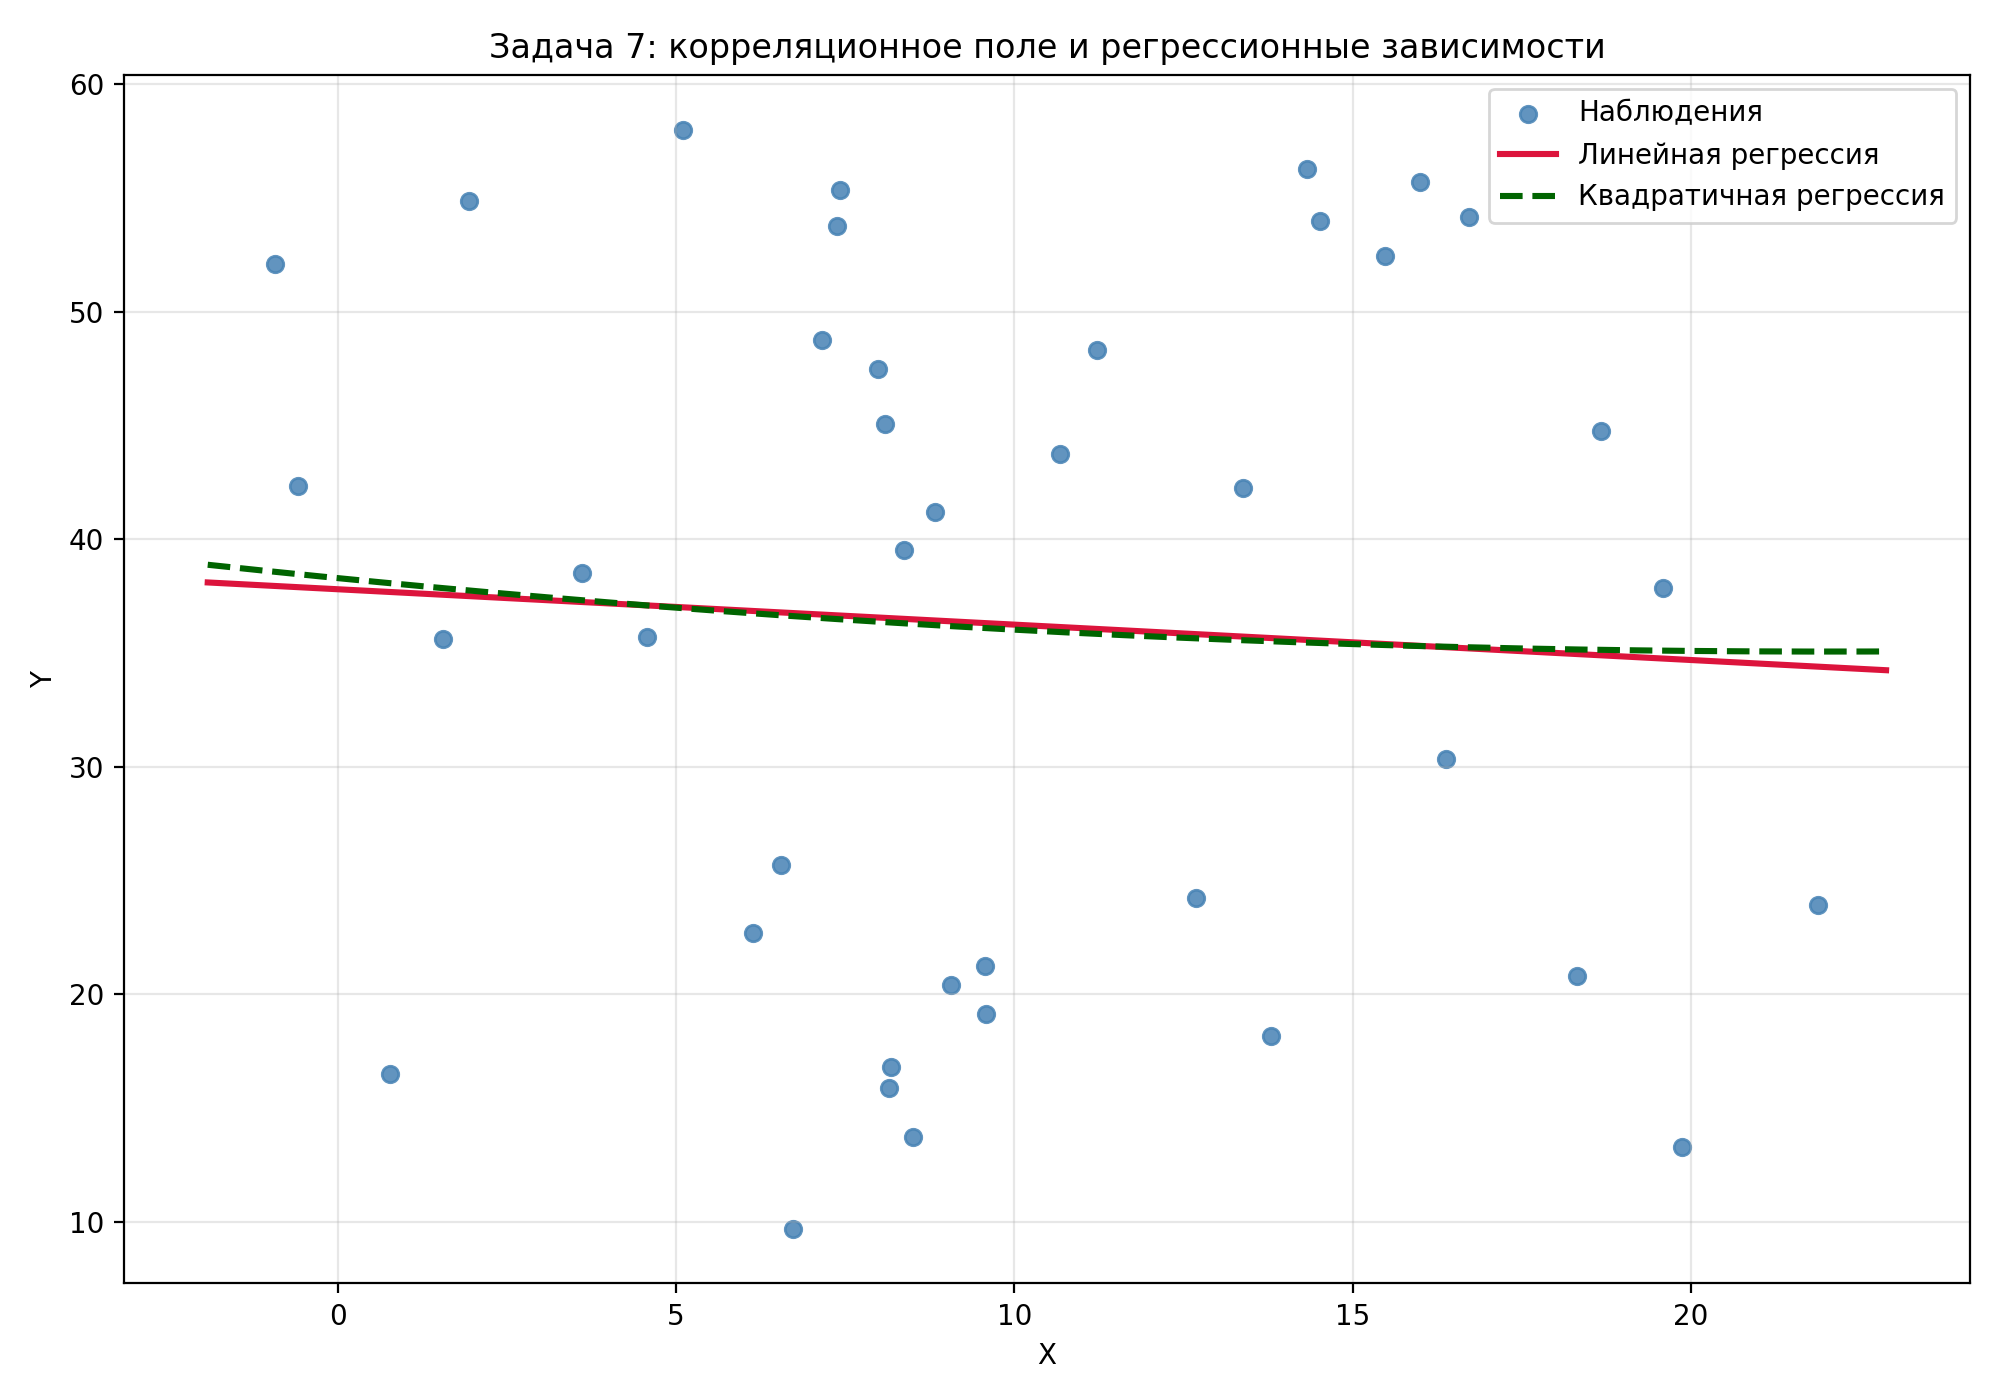
\includegraphics[width=\linewidth]{figures/task7_regression.png}
    \caption{Корреляционное поле и оценки линейной и квадратичной регрессии}
\end{figure}

\subsection*{Использованный код}

\begin{lstlisting}
A1 = np.column_stack([np.ones_like(x), x])
coef1, *_ = np.linalg.lstsq(A1, y, rcond=None)
pred1 = A1 @ coef1
sse1 = float(np.sum((y - pred1) ** 2))
s2_1 = sse1 / (n - 2)
r2_1 = 1 - sse1 / float(np.sum((y - y_mean) ** 2))

A2 = np.column_stack([np.ones_like(x), x, x**2])
coef2, *_ = np.linalg.lstsq(A2, y, rcond=None)
pred2 = A2 @ coef2
sse2 = float(np.sum((y - pred2) ** 2))
s2_2 = sse2 / (n - 3)
r2_2 = 1 - sse2 / float(np.sum((y - y_mean) ** 2))
\end{lstlisting}

\appendix
\section*{Приложение А. Данные варианта}

\subsection*{Таблица 1. Выборка для задачи 1}
\scriptsize
\setlength{\tabcolsep}{3pt}
\begin{longtable}{cccccccccc}
\caption{Приложение А, таблица 1. Выборка для задачи 1}\\
\toprule
1 & 2 & 3 & 4 & 5 & 6 & 7 & 8 & 9 & 10 \\
\midrule
\endfirsthead
\toprule
1 & 2 & 3 & 4 & 5 & 6 & 7 & 8 & 9 & 10 \\
\midrule
\endhead
0,11 & -1,53 & -0,94 & 0,21 & 0,77 & 1,10 & 0,23 & -0,15 & 0,79 & -0,71 \\
1,17 & 0,01 & 0,45 & 1,55 & 1,48 & -0,09 & 0,01 & 1,00 & 1,25 & 1,35 \\
0,52 & -1,61 & 2,16 & 0,64 & 0,19 & 0,02 & 0,20 & 1,43 & 0,74 & -0,21 \\
0,41 & 0,80 & -0,41 & 0,31 & -1,26 & 0,75 & 1,05 & 2,04 & -0,42 & -1,06 \\
0,33 & -0,30 & -0,34 & -0,10 & -1,54 & 0,67 & -0,40 & -0,15 & 0,98 & -1,04 \\
1,55 & -1,58 & 1,78 & -0,71 & 0,75 & 0,48 & -0,18 & 0,49 & -0,07 & 0,90 \\
1,04 & 2,75 & 1,03 & 0,76 & -2,53 & 0,27 & 0,92 & -1,17 & -0,85 & -1,83 \\
-0,35 & -1,07 & -0,02 & 1,64 & 0,35 & -0,86 & -0,06 & 0,69 & 2,16 & -0,54 \\
1,20 & -0,57 & 1,57 & -0,05 & 0,34 & 0,83 & -0,28 & 0,48 & 1,85 & 0,93 \\
0,91 & -1,50 & -1,08 & 0,53 & -0,53 & 0,29 & 0,77 & -1,13 & -0,76 & 2,30 \\
\bottomrule
\end{longtable}


\subsection*{Таблица 2. Выборка для задачи 3}
\scriptsize
\setlength{\tabcolsep}{3pt}
\begin{longtable}{c}
\caption{Приложение А, таблица 2. Выборка для задачи 3}\\
\toprule
$X_{16}$ \\
\midrule
\endfirsthead
\toprule
$X_{16}$ \\
\midrule
\endhead
3,02 \\
0,19 \\
10,23 \\
1,42 \\
20,05 \\
8,85 \\
30,27 \\
10,71 \\
19,97 \\
4,25 \\
16,37 \\
20,77 \\
8,81 \\
17,37 \\
13,78 \\
22,46 \\
7,26 \\
20,45 \\
17,57 \\
7,82 \\
16,86 \\
-2,40 \\
16,99 \\
13,49 \\
-0,45 \\
12,39 \\
8,68 \\
5,75 \\
14,54 \\
16,34 \\
6,14 \\
12,24 \\
2,39 \\
7,93 \\
0,12 \\
26,79 \\
\bottomrule
\end{longtable}


\subsection*{Таблица 3. Выборка для задачи 7}
\scriptsize
\setlength{\tabcolsep}{3pt}
\begin{longtable}{cc}
\caption{Приложение А, таблица 3. Выборка для задачи 7}\\
\toprule
$X$ & $Y$ \\
\midrule
\endfirsthead
\toprule
$X$ & $Y$ \\
\midrule
\endhead
8,50 & 13,74 \\
3,61 & 38,50 \\
11,22 & 48,30 \\
16,38 & 30,34 \\
15,99 & 55,70 \\
18,67 & 44,78 \\
-0,92 & 52,11 \\
8,83 & 41,22 \\
15,48 & 52,45 \\
4,57 & 35,70 \\
6,55 & 25,66 \\
1,55 & 35,63 \\
0,77 & 16,51 \\
5,11 & 58,01 \\
6,13 & 22,70 \\
-0,59 & 42,35 \\
7,16 & 48,75 \\
7,98 & 47,47 \\
10,67 & 43,74 \\
8,17 & 16,78 \\
8,37 & 39,54 \\
8,15 & 15,87 \\
16,71 & 54,16 \\
9,57 & 21,23 \\
9,07 & 20,42 \\
7,43 & 55,34 \\
19,86 & 13,29 \\
14,33 & 56,27 \\
21,88 & 23,90 \\
6,73 & 9,70 \\
18,31 & 20,82 \\
1,94 & 54,89 \\
12,69 & 24,21 \\
14,51 & 54,01 \\
19,59 & 37,85 \\
9,58 & 19,14 \\
7,38 & 53,79 \\
13,38 & 42,25 \\
8,09 & 45,05 \\
13,79 & 18,17 \\
\bottomrule
\end{longtable}



\end{document}
